\documentclass[../../main.tex]{subfiles}


\begin{document}
\subsection*{(a)}
We created the following OLAP Table:\\
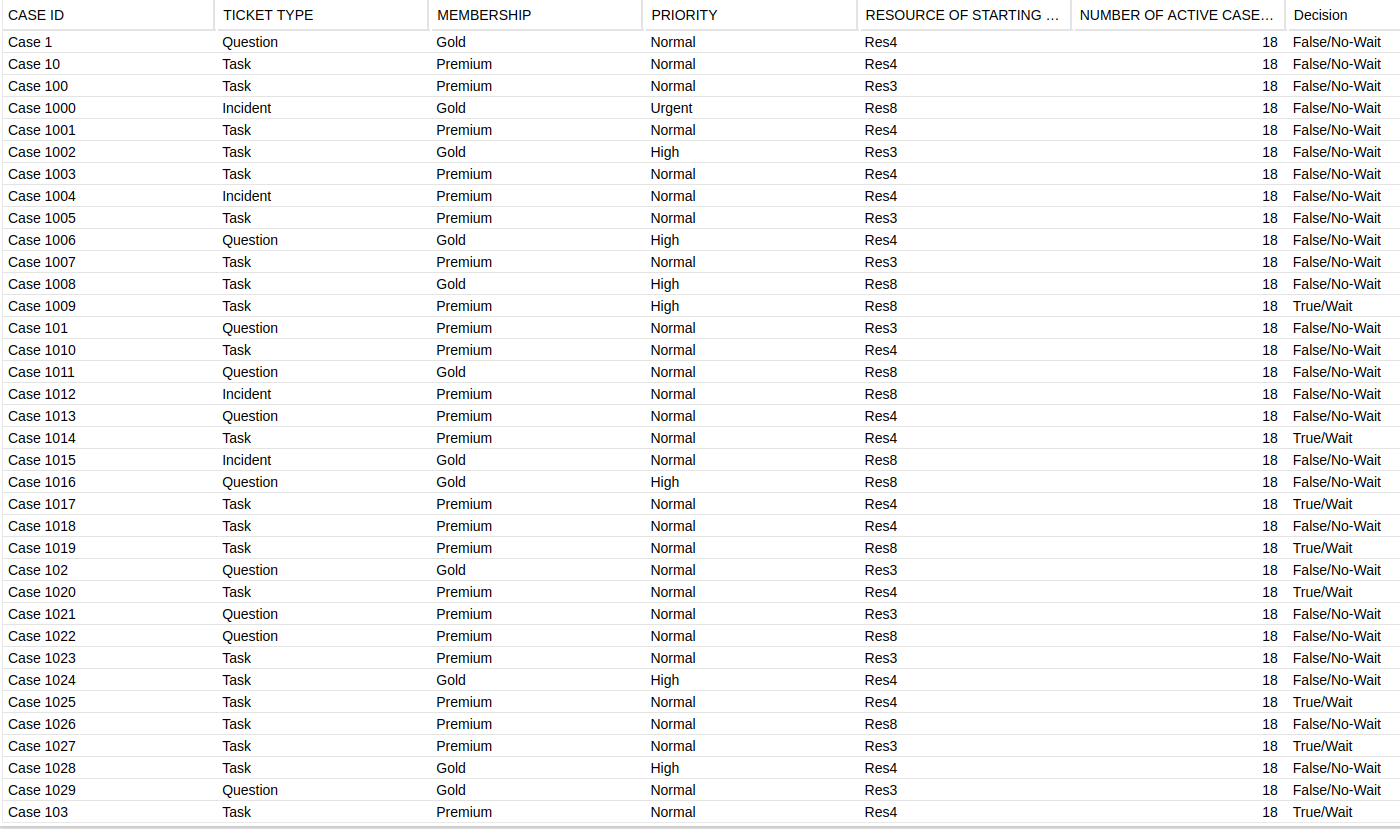
\includegraphics[width=\columnwidth]{img/Celonis_a_OLAP_Table.png}\\
For this, we used the following PQL Queries in the order of columns in the image left to right:
\begin{verbatim}
	"case_table_csv"."CASE ID"
\end{verbatim}
\begin{verbatim}
	"case_table_csv"."TICKET TYPE"
\end{verbatim}
\begin{verbatim}
	"event_table_csv"."PRIORITY"
\end{verbatim}
\begin{verbatim}
	PU_FIRST ( "case_table_csv", "event_table_csv"."RESOURCE")
\end{verbatim}
\begin{verbatim}
RUNNING_SUM (
  CASE WHEN MATCH_PROCESS_REGEX("event_table_csv"."ACTIVITY", 'Closed'$) = 1 THEN 0
  ELSE 1
  END
)
\end{verbatim}
\begin{verbatim}
CASE WHEN
	MATCH_PROCESS_REGEX ( "event_table_csv"."ACTIVITY", 'Wait' ) = 1 THEN 'True/Wait'
	ELSE 'False/No-Wait'
END
\end{verbatim}


\subsection*{(b)}
First, we export the OLAP Table and import it into RapidMiner as described in Instruction 2.
After setting the attribute Decision as our label, we had to adjust the minimal gain ratio to 0.006 in order to see more than just one Wait-Leaf. The resulting decision tree is evidently too large to fit into a PDF, thus we have added the description in the Appendix:
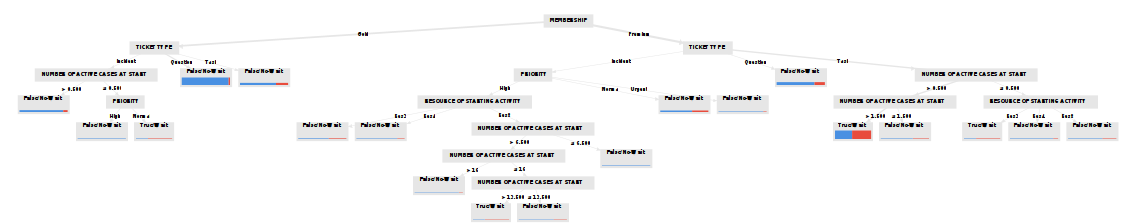
\includegraphics[width=\columnwidth]{img/RapidMiner_b_Decision_Tree.png}\\
We found that some tasks using Resource 3 would wait, even if they were the only task running at creation. From the tree we can also observe that some high priority incidents (using Resource 3 or 8) would have to wait depending on the number of active cases at start, although there does not seem to be any connection to the prior predictor variables.

After removing the attribute 'number of active cases at start' and further lowering the minimal gain ratio to 0.001, we get a much more simplified, but comprehensible Decision Tree:
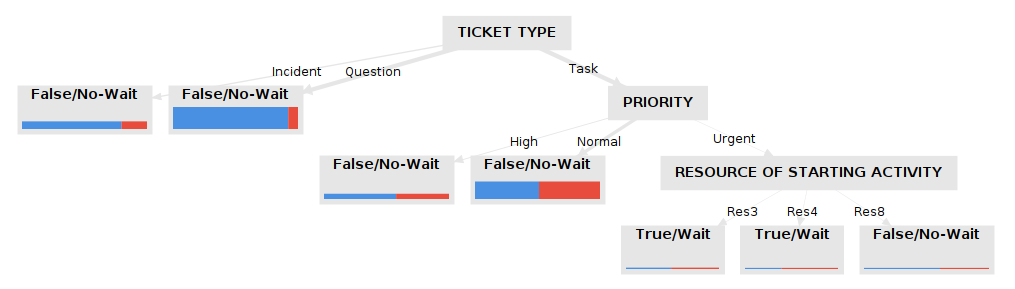
\includegraphics[width=\columnwidth]{img/RapidMiner_b_Decision_Tree_filtered.png}\\
Here we see that urgent tasks using the starting resource 3 or 4 are quite likely to be set into waiting mode.

\end{document}